\chapter{L'azienda}
\label{cap:lazienda}


\section\azienda

\subsection{Descrizione dell'Azienda}
Nata nel 1984, \azienda rappresenta oggi una realtà di primo piano nel panorama della consulenza e dello sviluppo software. 
Vanta un portfolio con oltre 2500 clienti, tra cui spiccano nomi di rilievo internazionale. \\
L'impegno verso la clientela è il pilastro su cui si fonda l'azienda, che si estende con uffici in molteplici 
regioni italiane: dal Veneto alla Lombardia, passando per Emilia-Romagna, Friuli-Venezia Giulia, Toscana, Puglia e 
Campania. Un team di oltre 600 professionisti, altamente qualificati, costituisce la forza lavoro di \azienda. \\
Il fulcro dell'innovazione è localizzato nel Centro di Sviluppo e Ricerca (CSV) a Grisignano di Zocco (VI). 
Qui, più di 200 tra sviluppatori e tecnici lavorano in sinergia per creare soluzioni software su misura, 
efficienti e affidabili, progettate per soddisfare le esigenze specifiche di ogni cliente. \\
\newpage

\subsection{Organizzazione e Prodotti}
L'organizzazione di \azienda è strutturata in diverse \textit{Business Unit} (BU), ciascuna con una visione, \textit{mission}, obiettivi e strategie specifici. Operando in modo autonomo o semi-autonomo, queste unità hanno una struttura organizzativa propria e sono responsabili dei loro bilanci economici, permettendo una focalizzazione mirata su mercati geografici, gruppi di clienti o linee di prodotto specifici. Questa struttura rende \azienda agile e reattiva alle dinamiche di mercato. \\
Le BU in \azienda sono 11, distinte per aree di specializzazione, come illustrato in figura \ref{fig:organizzazione-azienda}:
\begin{itemize}
\item \textbf{JGALILEO:} offre l’\gls{ERP} Jgalileo, un sistema di gestione integrato che ottimizza i processi aziendali per imprese di varie dimensioni, con un focus sulle normative fiscali internazionali;
\item \textbf{NEXTBI:} si concentra su \textit{Information Technology} e consulenza strategica, specializzandosi in \textit{marketing}, vendite, \textit{retail}, innovazione cliente, Business Intelligence e soluzioni \gls{IoT};
\item \textbf{4WORDS:} fornisce soluzioni \gls{B2B}, app e \gls{CRM}, per potenziare il \textit{business} attraverso strumenti digitali, inclusi portali B2B e realtà aumentata;
\item \textbf{TCE:} si dedica alla semplificazione delle fasi di preventivazione e acquisizione ordini con il prodotto \gls{CPQg};
\item \textbf{DISCOVERY QUALITY:} sviluppa software per la \textit{Governance} aziendale, controllo dei processi e misurazione delle performance, con un occhio alle normative e metriche di sostenibilità (\gls{SDGs}, \gls{BCorp});
\item \textbf{ECM:} propone soluzioni di \gls{ECM} per la gestione efficace dei documenti digitali;
\item \textbf{SMITECH:} focalizzata sulla \textit{\gls{cybersecurity}} e protezione dei dati;
\item \textbf{ELEMENT:} è la divisione creativa per lo sviluppo di siti web ed e-commerce, con un focus sull'esperienza utente;
\item \textbf{JPA:} sviluppa software di \gls{BPM} per l'automazione e integrazione dei processi aziendali;
\item \textbf{FACTORY:} risponde alle esigenze della \gls{Supply Chain} con soluzioni per la fabbrica del futuro, mirate a ottimizzare servizio clienti, asset e profitti;
\item \textbf{JPM:} offre soluzioni di \textit{\gls{Project Management}} per la gestione di progetti complessi.
\end{itemize}

\newpage

\subsection{Strategie e Obiettivi}
Il piano strategico triennale di \azienda, denominato \textit{Vision 2025}, mira alla crescita sostenibile, all'innovazione costante e alla soddisfazione del cliente. \\
L'obiettivo principale è espandere la penetrazione di mercato sia in Italia che all'estero, consolidando la presenza nei mercati esistenti e esplorando nuovi orizzonti internazionali, con un focus particolare sul mercato nordamericano e asiatico. \\
Per realizzare questa visione, \azienda investe in tecnologie avanzate e nel potenziamento delle competenze dei suoi team, oltre a implementare un modello operativo più efficiente e flessibile. \\
Un altro obiettivo è promuovere la responsabilità sociale d'impresa, impegnandosi nel rispetto dei \gls{SDGs} e perseguendo la certificazione \gls{BCorp}, a testimonianza di un impatto positivo sia sociale che ambientale. \\
Infine, \azienda prevede di ampliare il proprio portafoglio prodotti con soluzioni innovative e di migliorare continuamente la qualità e le performance dei prodotti esistenti, per assicurare ai clienti il massimo valore aggiunto.


\begin{figure}[!h] 
  \centering 
  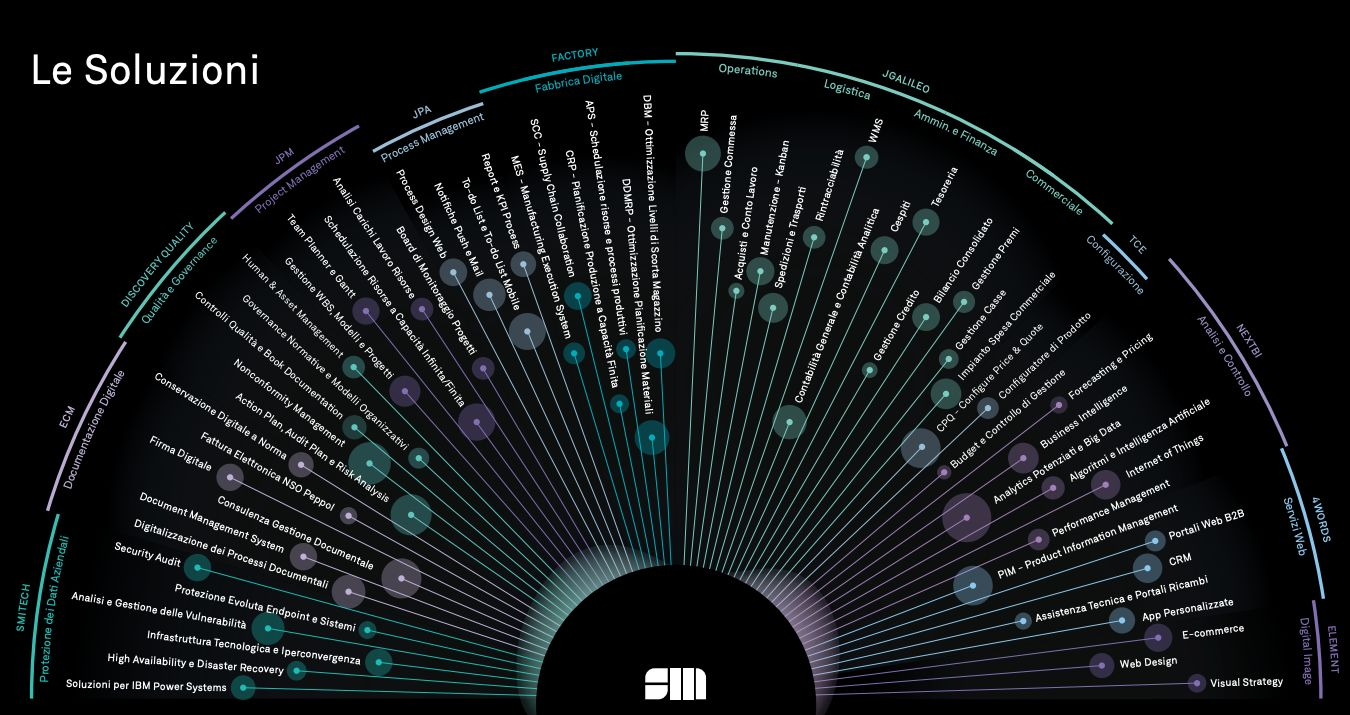
\includegraphics[width=1\columnwidth]{organizzazione-azienda} 
  \caption{Le BU di {\azienda} ed i loro prodotti}
  \label{fig:organizzazione-azienda}
\end{figure}

\noindent La Business Unit (BU) incarna il principio dello sviluppo agile, che privilegia la collaborazione, 
la flessibilità e la consegna incrementale di valore nel corso del progetto. 
\\Questo approccio enfatizza l'importanza di rispondere rapidamente ai cambiamenti piuttosto che seguire rigidamente un piano prestabilito. 
\\In questo contesto agile, ogni progetto è supervisionato da un responsabile che gestisce il \textit{budget} e le risorse umane,
 elementi cruciali per il dinamismo e l'adattabilità richiesti.

\noindent Ogni progetto all'interno della BU è supportato da un team di professionisti diversificati, i cui ruoli sono descritti come segue:
\begin{itemize}
\item Un \gls{PO} che ha il compito di guidare il progetto, fungendo da collegamento critico tra il team di sviluppo e il cliente;
\item Uno \gls{Scrum Master} che è responsabile del mantenimento dell'efficienza del team di sviluppo, 
promuovendo e facilitando le metodologie agili;
\item Gli sviluppatori, che rappresentano la forza creativa dietro allo sviluppo del prodotto;
\item I tester, incaricati di assicurare che il prodotto funzioni correttamente attraverso test approfonditi;
\item I consulenti, che agiscono come mediatori con il cliente, comprendendo le sue necessità e configurando il prodotto in base a queste;
\item Gli \gls{analisti}, che analizzano i requisiti del cliente e preparano la documentazione necessaria, spesso assumendo ruoli aggiuntivi come sviluppatori o tester.
\end{itemize}

\noindent Questa configurazione enfatizza l'importanza di una gestione strategica e di una collaborazione integrata per il successo dei progetti e la crescita della BU.






\noindent In aggiunta alle componenti precedentemente descritte, ci sono anche altre figure che compongono l'azienda:
\begin{itemize}
  \item \textbf{HR:} si occupa di gestire le risorse umane, di reclutare nuovi dipendenti e di gestire i rapporti con i dipendenti;
  \item \textbf{Marketing:} si occupa di gestire il sito web, i social network e di creare materiale pubblicitario;
  \item \textbf{Amministrazione:} si occupa di gestire la contabilità e le risorse economiche;
  \item \textbf{IT:} si occupa di gestire l'infrastruttura informatica e di fornire supporto ai dipendenti;
  \item \textbf{Commerciali:} si occupano di trovare nuovi clienti e di gestire i rapporti con i clienti esistenti;
  \item \textbf{Direzione:} si occupa di gestire l'azienda e di prendere decisioni strategiche;
  \item \textbf{Centralino:} si occupa di gestire le telefonate e di accogliere i clienti;
  \item \textbf{Presidente:} fondatore dell'azienda, si occupa di prendere decisioni strategiche e di gestire i rapporti con i clienti più importanti;
  \item \textbf{Amministratore delegato:} si occupa di gestire l'azienda e di prendere decisioni strategiche;
\end{itemize}

All'interno dell'azienda c'è una parte di dipendenti che lavora in sede, una parte che lavora in remoto e una parte che lavora presso i clienti. \\
Per riuscire a monitorare il lavoro di tutti i dipendenti, l'azienda utilizza un software di \textit{time tracking} che permette di registrare le ore lavorate. \\
Ogni dipendente ha un proprio \textit{account} che permette di registrare le ore lavorate, di richiedere ferie e permessi. \\
Il software permette di visualizzare le ore lavorate da ogni dipendente e di generare report per ogni progetto e per ogni cliente. \\
Durante l'inserimento delle ore lavorate (Rapporino), il dipendente deve inserire una descrizione delle attività svolte, la commessa, l'eventuale cliente,
la sede in cui ha lavorato, l'ora di inizio e fine lavoro ed eventualmente può collegare il Rapporino ad un ticket. \\
Questa operazione deve essere fatta per ogni giorno lavorativo e ad ogni chiusura del mese vengono bloccate le ore lavorate. \\

\newpage

\section{Il team di sviluppo}
Il team di sviluppo in cui ho lavorato fa parte della BU \textit{JPA} (\textit{Process Management}) e non si
occupa di sviluppare un prodotto specifico, ma ha come obiettivo quello di fornire supporto a tutti i team di sviluppo
dell'azienda. \\
Le principali attività del team sono le seguenti:
\begin{itemize}
  \item \textbf{Supporto:} il team fornisce supporto ai team di sviluppo per la risoluzione di problemi tecnici e analitici;
  \item \textbf{Formazione:} il team fornisce formazione ai team di sviluppo per l'utilizzo di nuovi strumenti e tecnologie;
  \item \textbf{Ricerca e sviluppo:} il team si occupa di sviluppare un \textit{\gls{frameworkg}} interno che permette di creare applicazioni web in modo semplice e veloce;
  \item \textbf{Automazione:} il team si occupa di automatizzare i processi di sviluppo, come ad esempio la compilazione, il rilascio di un prodotto o lo sviluppo di uno nuovo; 
  \item \textbf{Gestione repository:} il team si occupa di gestire i repository di codice sorgente e di fornire supporto per l'utilizzo di strumenti di \textit{\gls{continuous_integrationg}};
  \item \textbf{Installatore:} il team si occupa di sviluppare un installatore per i prodotti dell'azienda che utilizzano il \textit{\gls{frameworkg}} interno;
\end{itemize}

\noindent Il team è composto da 3 persone, uno \gls{Scrum Master} e due sviluppatori. \\
In questo caso sviluppatori sono anche analisti e tester, e molto spesso anche lo \gls{Scrum Master} 
partecipa alle analisi tecniche e funzionali. \\


\section{Strumenti utilizzati}
I principali strumenti per lo sviluppo da me utilizzati sono stati i seguenti:\\
\begin{itemize}
  \item \textbf{Intellij IDEA:} un ambiente di sviluppo integrato (\gls{IDEg}) per il linguaggio di programmazione Java. Fornisce strumenti e funzionalità avanzate per supportare lo sviluppo efficiente del codice, il debug e la testing. Con la sua interfaccia user-friendly e le potenti funzionalità, come l'analisi statica del codice e il refactoring intelligente, IntelliJ IDEA è scelto da molti sviluppatori per creare applicazioni Java professionali;
  \item \textbf{WebStorm:} un IDE per lo sviluppo di applicazioni web, che fornisce un'esperienza di sviluppo ottimale. Grazie alla sua integrazione con strumenti di supporto per lo sviluppo web, come \textit{Node.js}, \textit{Angular}, \textit{React}, WebStorm permette di sviluppare applicazioni web moderne con facilità;
  \item \textbf{Neo4j Desktop:} un programma che permette di installare e gestire database \textit{Neo4j} in modo semplice e veloce. Permette di creare e gestire più database, di monitorare le performance e di eseguire query;
  \item \textbf{Git:} un sistema di controllo versione distribuito, utilizzato per il versionamento del codice sorgente; 
  \item \textbf{Gradle:} un sistema di automazione open source che gestisce le dipendenze e permette di automatizzare il processo di compilazione, testing, pubblicazione e deployment di un software;
  \item \textbf{Docker:} un progetto open source che automatizza il deployment di applicazioni all'interno di contenitori software, fornendo un'astrazione aggiuntiva grazie alla virtualizzazione a livello di sistema operativo di Linux;
  \item \textbf{Bitbucket:} un servizio di hosting per progetti che utilizzano Git come sistema di controllo versione. Fornisce strumenti per la collaborazione e la gestione del codice sorgente;
  \item \textbf{Jenkins:}  un software open source che permette di automatizzare il processo di \textit{build}, testing e deployment di un software;
  \item \textbf{Angular:} un {\gls{frameworkg}} open source per lo sviluppo di applicazioni web, scritto in TypeScript. 
  Fornisce un'architettura \gls{mvvm} e permette di creare applicazioni web dinamiche e scalabili;
  \item \textbf{Jira:} un software di tracciamento dei bug e gestione dei progetti, che permette di pianificare, monitorare e rilasciare software di qualità;
  \item \textbf{Confluence:} un software di collaborazione che permette di creare, organizzare e discutere documenti di progetto;
\end{itemize}

I linguaggi utilizzati sono i seguenti:\\

\begin{itemize}
  \item \textbf{Java:} un linguaggio di programmazione ad alto livello, orientato agli oggetti e a tipizzazione statica, che permette di creare applicazioni web, desktop e mobile;
  \item \textbf{Javascript:} un linguaggio di programmazione ad alto livello, orientato agli oggetti e a tipizzazione dinamica, che permette di creare applicazioni web dinamiche;
  \item \textbf{TypeScript:} un super-set di Javascript che permette di aggiungere tipizzazione statica al linguaggio;
  \item \textbf{Groovy:} un linguaggio di programmazione che permette di scrivere codice che viene eseguito sulla \gls{JVM};
  \item \textbf{Chyper:} un linguaggio di query dichiarativo per grafi, utilizzato per interrogare database \gls{Neo4j};
\end{itemize}

\subsection{Convenzioni}
Per lo sviluppo dei progetti che utilizzano il \textit{frameworkg} interno, sono state definite delle convenzioni da seguire.
Le convenzioni sono salvate all'interno di Confluence, in modo da essere facilmente accessibili a tutti i dipendenti. \\
Sono divise nelle seguenti categorie:
\begin{itemize}
  \item \textbf{Documentazione:} sono delle regole che indica come documentare il codice sorgente, in modo da facilitare la comprensione del codice;
  \item \textbf{Scrittura analisi:} sono delle regole che indicano come scrivere l'analisi dei requisiti e le strutture dell basi di dati, in modo da facilitare la comprensione dell'analisi;
  \item \textbf{Progettazione:} sono delle regole che indicano come progettare i componenti software, in modo da facilitare la manutenzione e l'estensione del codice;
  \item \textbf{Codifica:} sono delle regole che permettono di scrivere codice in modo uniforme, in modo da facilitare la lettura e la comprensione del codice;
  \item \textbf{Versionamento:} sono delle regole che indicano come versionare il codice sorgente, in modo da facilitare la ricerca di una versione specifica del codice;
\end{itemize}

\newpage
\section{Rapporto con l'innovazione}

{\azienda} ha come obiettivo l’innovazione delle aziende clienti per contribuire al loro progresso, 
agevolando la trasformazione digitale ed è specializzata nella progettazione e nella realizzazione di soluzioni integrate, 
a supporto della riorganizzazione di tutti i processi aziendali e professionali.\\
Per raggiungere questo obiettivo, l'azienda indirizza ogni anno dal 15 al 20\% del proprio fatturato all’attività di Ricerca e Sviluppo.\\
Uno dei punti di forza di {\azienda} è la capacità di cogliere le idee e i suggerimenti dei clienti, dei dipendenti, dei collaboratori e trarne ispirazione per sviluppare nuovi prodotti e nuove soluzioni.\\
In questo momento quasi tutti i prodotti attualmente installati presso i clienti hanno una nuova versione in fase di sviluppo,
questo permette all'azienda di essere sempre all'avanguardia e di fornire ai clienti prodotti sempre aggiornati.\\
\\
L'azienda punta molto alla cultura e alla formazione dei propri dipendenti, 
infatti ogni anno vengono organizzati corsi di formazione per permettere ai dipendenti di imparare nuove tecnologie e nuovi strumenti.\\
Questi corsi sono tenuti da dipendenti dell'azienda che hanno già esperienza con le tecnologie e gli strumenti trattati, da consulenti esterni 
o tramite \textit{e-learning}, sulla piattaforma \textit{Udemy Business} messa a disposizione gratuitamente dall'azienda.\\
\\
Inoltre, l'azienda organizza molti eventi dedicati all'innovazione, come ad esempio \textit{Choose Innovation} in collaborazione con \textit{IBM},
dove i vari relatori discutono di innovazione e di come le aziende possono innovare.\\